\documentclass[a4paper,
fontsize=11pt,
%headings=small,
oneside,
numbers=noperiodatend,
parskip=half-,
bibliography=totoc,
final
]{scrartcl}

\usepackage{synttree}
\usepackage{graphicx}
\setkeys{Gin}{width=.6\textwidth} %default pics size

\graphicspath{{./plots/}}
\usepackage[ngerman]{babel}
\usepackage[T1]{fontenc}
%\usepackage{amsmath}
\usepackage[utf8x]{inputenc}
\usepackage [hyphens]{url}
\usepackage{booktabs} 
\usepackage[left=2.4cm,right=2.4cm,top=2.3cm,bottom=2cm,includeheadfoot]{geometry}
\usepackage{eurosym}
\usepackage{multirow}
\usepackage[ngerman]{varioref}
\setcapindent{1em}
\renewcommand{\labelitemi}{--}
\usepackage{paralist}
\usepackage{pdfpages}
\usepackage{lscape}
\usepackage{float}
\usepackage{acronym}
\usepackage{eurosym}
\usepackage[babel]{csquotes}
\usepackage{longtable,lscape}
\usepackage{mathpazo}
\usepackage[flushmargin,ragged]{footmisc} % left align footnote

\usepackage{listings}

\urlstyle{same}  % don't use monospace font for urls

\usepackage[fleqn]{amsmath}

%adjust fontsize for part

\usepackage{sectsty}
\partfont{\large}

%Das BibTeX-Zeichen mit \BibTeX setzen:
\def\symbol#1{\char #1\relax}
\def\bsl{{\tt\symbol{'134}}}
\def\BibTeX{{\rm B\kern-.05em{\sc i\kern-.025em b}\kern-.08em
    T\kern-.1667em\lower.7ex\hbox{E}\kern-.125emX}}

\usepackage{fancyhdr}
\fancyhf{}
\pagestyle{fancyplain}
\fancyhead[R]{\thepage}

%meta
%meta

\fancyhead[L]{U. Jung \\ %author
LIBREAS. Library Ideas, 26 (2014). % journal, issue, volume.
\href{http://nbn-resolving.de/urn:nbn:de:kobv:11-100219254
}{urn:nbn:de:kobv:11-100219254}} % urn
\fancyhead[R]{\thepage} %page number
\fancyfoot[L] {\textit{Creative Commons BY 3.0}} %licence
\fancyfoot[R] {\textit{ISSN: 1860-7950}}

\title{\LARGE{Abstand als Alternative? Vom Normalen und weniger Normalen in kamerunischen Bibliotheken}} %title %title
\author{Uwe Jung} %author

\setcounter{page}{}

\usepackage[colorlinks, linkcolor=black,citecolor=black, urlcolor=blue,
breaklinks= true]{hyperref}

\date{}
\begin{document}

\maketitle
\thispagestyle{fancyplain} 

%abstracts
\begin{abstract}
Am praktischen Beispiel des kamerunischen Bibliothekswesens werden
Probleme bei der Übernahme von ``traditionellen'' Bibliothekskonzepten
in andere Kulturen verdeutlicht. Die Lösungen dieser Probleme werden zum
einen in einem besseren Verständnis der handelnden Akteure, zum anderen
in einer Neuausrichtung der Zusammenarbeit mit eben diesen Akteuren
gesehen.
\end{abstract}

%body
\section*{Ein Anfang}\label{ein-anfang}

Wer nach alternativen Bibliothekskonzepten fragt, muss sich zunächst
über das Wesen traditioneller Bibliothekskonzepte im Klaren sein. Diese
Frage scheint für weite Teile Europas und Nordamerikas geklärt zu sein.
Doch in einem Land, in welchem der konstruierte Widerspruch zwischen
Tradition und Moderne regelmäßig unter wechselnden Vorzeichen betrachtet
wird, ist dies weniger klar, als gemeinhin angenommen. Der nachfolgende
Text entstand als Ergebnis langjähriger aktiver Beobachtung in der
bibliothekarischen Praxis Kameruns. Obgleich er versucht, einige der
beschriebenen Phänomene ansatzweise theoretisch zu unterlegen, erhebt er
doch keinen Anspruch auf eine umfassende theoretische Erklärung.

Kamerun liegt an der Grenze zwischen West- und Zentralafrika. Das Land
war zwischen 1884 und 1916 eine deutsche Kolonie. Mehr noch, während
dieser Zeit wurden dutzende von verschiedenen lokalen Gesellschaften
zwischen Atlantik und Tschadsee unter einer zentralen Verwaltung
zusammengefasst. Wichtigstes Erbe dieser gemeinsamen Geschichte war
folglich die Schaffung eines Staatswesens, dessen Name und dessen
Grenzen im Wesentlichen noch heute existieren. Nach dem 1. Weltkrieg
wurde das Land in zwei von Großbritannien und Frankreich verwaltete
Mandatsgebiete aufgeteilt, zunächst im Namen des Völkerbundes, später im
Namen der Vereinten Nationen. Dieses Doppelmandat führte unter anderem
dazu, dass die heutige Republik Kamerun in einen dominanten frankophonen
und einen kleineren anglophonen Landesteil unterteilt ist. Anfang der
1960er Jahre wurden beide Mandatsgebiete, euphemistisch ausgedrückt, in
die politische Unabhängigkeit entlassen. Das zunächst föderalistisch
geprägte System wurde 1972 zugunsten eines zentralistischen
Einheitsstaates abgeschafft.

\begin{figure}[htbp]
\centering
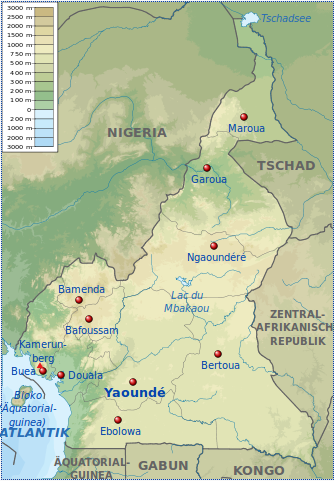
\includegraphics{img/KarteKamerun.png}
\caption{Übersichtskarte Kamerun. Kamerun ist in zehn Regionen
unterteilt. Die größten Städte sind Duala, Jaunde und Bafoussam.
Bildquelle: \url{http://de.wikipedia.org/wiki/Kamerun} CC-BY-SA.}
\end{figure}

\begin{figure}[htbp]
\centering
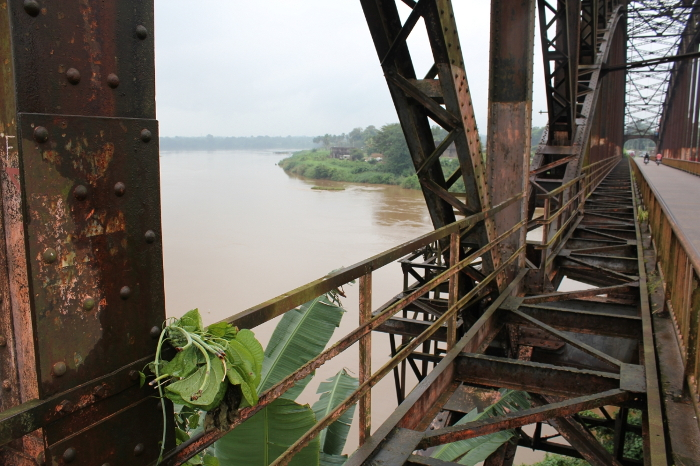
\includegraphics{img/BruckeEdea.jpg}
\caption{Eine alte Eisenbahnbrücke in Edea. Die 162 m lange Brücke über
den Sanaga stellt das vielleicht bekannteste, heute noch vorhandene
Bauwerk aus der deutschen Kolonialzeit dar. Bildquelle: Foto des
Autors.}
\end{figure}

\begin{figure}[htbp]
\centering
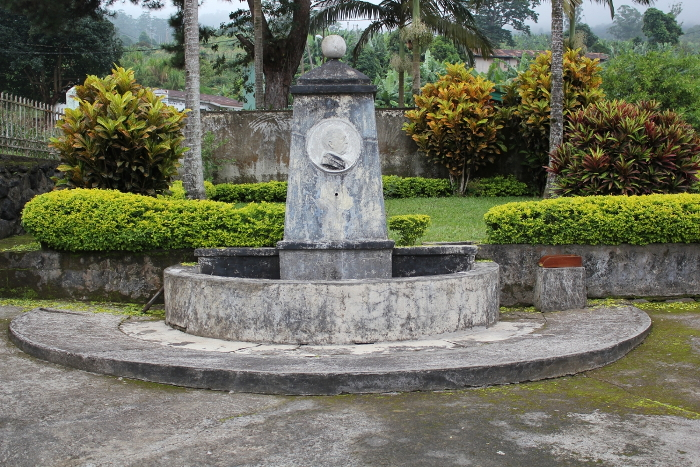
\includegraphics{img/Bismarckbrunnen.jpg}
\caption{Bismarck in den Tropen. Von der allgemeinen Bismarck-Euphorie
gegen Ende des 19. Jhs. blieb auch Kamerun nicht verschont. Der
Bismarck-Brunnen in Buea wurde 1899 vom damaligen Bezirksamtmann
Leuschner initiiert, der das Portrait gar eigenhändig modellierte
(Deutsches Kolonialblatt 1899, S. 368). Just im Rücken des Fotografen
befindet sich die Außenstelle Buea des Nationalarchivs, Standort eines
Teils der ehemaligen deutschen Gouvernements- Bibliothek. Bildquelle:
Foto des Autors.}
\end{figure}

\begin{figure}[htbp]
\centering
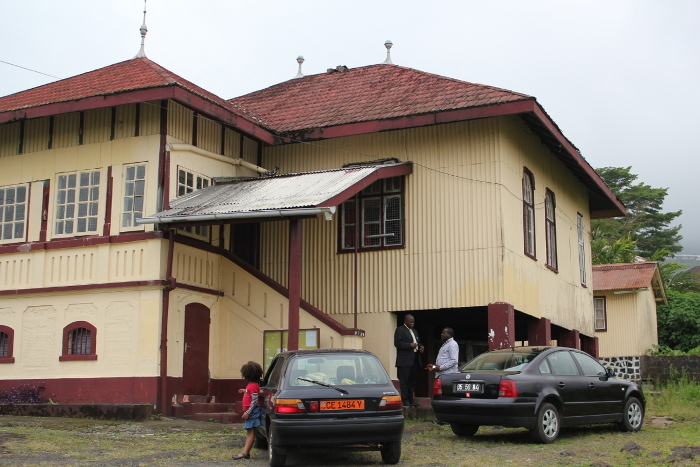
\includegraphics{img/MINACBuea.jpg}
\caption{Kolonialbauten in Buea. In diesem vor 1914 fertiggestellten
Gebäude residiert heute die regionale Verwaltung des Kulturministeriums
für die South-West-Region, eine von zwei anglophonen Regionen des
Landes. Bildquelle: Foto des Autors.}
\end{figure}

Die gegenwärtige politische Situation ist durch die seit 1982 währende
Amtszeit von Paul Biya gekennzeichnet. Unter dessen Ägide wurde eine
gewisse innenpolitische Stabilität durchgesetzt, die jedoch gleichzeitig
zu einer weitgehenden gesellschaftlichen Stagnation führte. Weitaus
problematischer ist jedoch die sich daraus ableitende
Zukunftsperspektive. Beobachter gehen derzeit davon aus, dass die
aktuelle politische Situation im Zusammenhang mit dem demnächst
anstehenden, jedoch offenbar unvorbereiteten Führungswechsel zu
gewaltsam ausgetragenen Konflikten führen wird.\footnote{International
  Crisis Group (ed.): \emph{Cameroon: Prevention is Better than Cure}.
  Africa Briefing N°101, 4 September 2014
  \url{http://www.crisisgroup.org/en/regions/africa/central-africa/cameroon.aspx}
  (besucht am 11.10.2014).}

\begin{figure}[htbp]
\centering
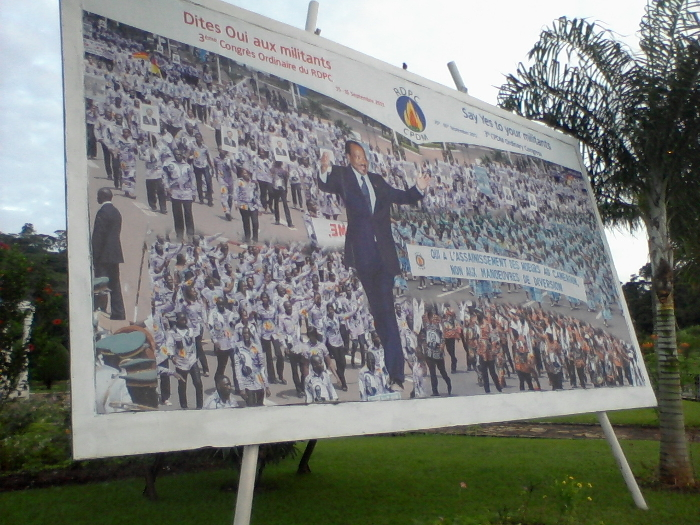
\includegraphics{img/Biya.jpg}
\caption{Ein Propaganda-Poster. Das Poster wurde 2011 anlässlich eines
Kongresses der regierenden Staatspartei RDPC aufgestellt. Übergroß im
Vordergrund: Paul Biya. Bildquelle: Foto des Autors.}
\end{figure}

Die letzten 130 Jahre haben im Gebiet des heutigen Kameruns zweifellos
tiefgreifende gesellschaftliche Veränderungen hervorgebracht. Es ist
wichtig, darauf hinzuweisen, dass diese Veränderungen zumeist auf das
Wirken äußerer Faktoren zurückzuführen sind. Landläufig wird für diese
Veränderungen oftmals der Begriff der Modernisierung verwendet. Jedoch
ist dieser Begriff gleich in mehrfacher Hinsicht problematisch. Weder
gibt es eine lineare Abfolge gesellschaftlicher Entwicklung vom
\enquote{Niederen} zum \enquote{Höheren}, noch gibt es einen klar
voneinander abzugrenzenden Gegensatz zwischen Tradition und
Moderne.\footnote{Zum Problem der Modernisierung von Gesellschaften gibt
  es verschiedene Denkrichtungen und eine umfangreiche Literatur. Von
  besonderer Bedeutung ist hierbei das Theoriensystem des
  Postkolonialismus. Siehe hierzu auch: Kerner, Ina: \emph{Postkoloniale
  Theorien zur Einführung}. Hamburg 2012-} Ist mit Modernisierung gar
gemeint, eine Gesellschaft nach aktuellen westlichen Maßstäben zu
entwickeln, wird der Begriff nicht mehr tragbar. Die besagten
Veränderungen haben in Kamerun vielmehr zu einer spezifischen
kamerunischen Gesellschaft mit eigenen Werten und Formen des
Zusammenlebens geführt. Dies zu erkennen, ist eine wichtige
Voraussetzung dafür, sich lernend mit einzelnen Institutionen und
Phänomenen dieser Gesellschaft beschäftigen zu können.

Das Spezifische der kamerunischen Gesellschaft führt jedoch zugleich zur
Feststellung, dass jede Form von Verallgemeinerung höchst problematisch
ist. Für Kamerun geltende Aussagen können nicht ohne weiteres auf eine
\enquote{afrikanische} Gesellschaft übertragen werden. Das Konstrukt
\enquote{Afrika} taugt nur bedingt zum Erkenntnisgewinn. Es musste
hingegen bereits zu oft als Vehikel für unzutreffende
Verallgemeinerungen herhalten. Das Ergebnis dessen lässt sich
sarkastisch zu dem Klischee vom Katastrophenkontinent mit fröhlich
tanzenden Bewohnern, phantastischen Landschaften und wilden Tieren
zusammenfassen. Oder, wie es der kenianische Schriftsteller Binyavanga
Wainaina sehr pointiert ausgedrückt hat: \enquote{Afrika ist der einzige
Kontinent, den man lieben kann.}\footnote{Binyavanga Wainaina:
  \emph{Hungersnöte sind gut. Über Afrika schreiben -- eine ironische
  Anleitung}. In: Fluter. Online-Ausgabe vom 1.2.2006
  \url{http://www.fluter.de/de/afrika/thema/4704/} (besucht am
  29.09.2014).}

\begin{figure}[htbp]
\centering
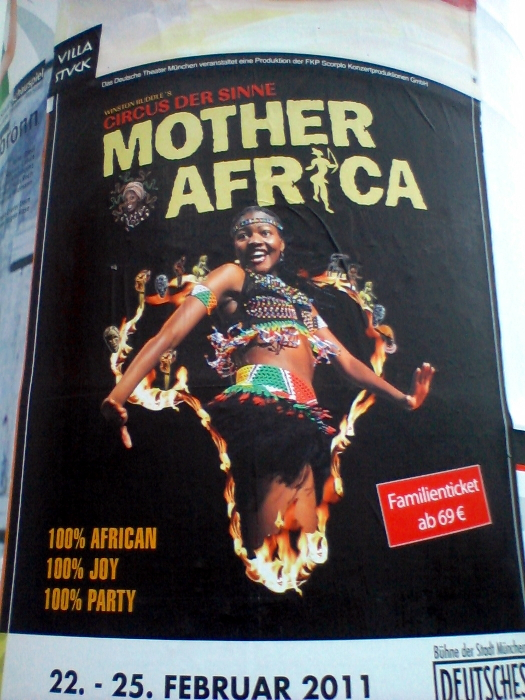
\includegraphics{img/Klischee.jpg}
\caption{Ein Veranstaltungsplakat in München. Klischees beherrschen die
Vorstellung über \enquote{Afrika} in Europa. Die hier vor der
obligatorischen Afrika-Karte dargestellte Dame trägt imitierten
\enquote{traditionellen} Glasperlen-Schmuck, übrigens ein typisches
koloniales Handelsprodukt im 18. und 19. Jahrhundert. Bildquelle: Foto
des Autors.}
\end{figure}

\section*{Bibliotheken in Kamerun}\label{bibliotheken-in-kamerun}

Bibliotheken in Kamerun sind fast immer unter dem Gesichtspunkt von
kolonialen und neokolonialen Auseinandersetzungen zu betrachten. Sie
entstanden und entstehen in den allermeisten Fällen auf der Basis eines
importierten und für allgemeingültig angesehenen Konzepts. Diese Aussage
gilt teilweise sogar für die berühmte vom König Njoya entwickelte
Bamum-Literatur, welche zu einem Zeitpunkt entstand, als die deutsche
Kolonialverwaltung bereits im Lande wirkte.\footnote{Sultan Njoya von
  Bamum (Fumban) begann Ende des 19 Jh. mit der Entwicklung eines
  eigenen Schriftsystems, der sogenannten Bamum-Schrift. Der direkte
  Kulturkontakt mit der deutschen Kolonialadministration erfolgte erst
  einige Jahre später. Es kann jedoch davon ausgegangen werden, dass
  Njoya bereits zu Beginn dieses Prozesses über die Bedeutung von
  Schrift als Mittel zur kolonialen Herrschaftssicherung einigermaßen
  informiert war. Michael Everson and Charles Riley: \emph{Preliminary
  proposal for encoding the Bamum script in the BMP of the UCS}. 2007
  \url{http://std.dkuug.dk/jtc1/sc2/wg2/docs/n3209.pdf} (besucht am
  11.10.2014).}

Eine der ersten traditionellen (oder sollte man hier besser sagen,
modernen) Bibliotheken in Kamerun entstand mit dem Aufbau der deutschen
Kolonialverwaltung ab 1884. Teile dieser sogenannten
Gouvernements-Bibliothek haben sich bis heute in Buea und
Jaunde\footnote{Im Text werden die Geografika konsequent in deutscher
  Schreibweise wiedergegeben, falls hierfür eine amtliche Übersetzung
  vorliegt. Es sollte aber klar sein, dass sowohl diese, als auch die
  aktuellen französischen und englischen Schreibweisen Produkte
  kolonialer Verwaltung darstellen. Teilweise existieren lokale
  Bezeichnungen, wie z.~B. Ongola für Jaunde (Yaoundé, Yaounde). Jedoch
  verbergen sich auch dahinter koloniale Phänomene und sind diese
  international nicht gebräuchlich.} erhalten. Dieser wahrscheinlich
ersten \enquote{europäischen} Bibliothek sollten noch weitere folgen.
Sie befinden sich hauptsächlich in Schulen und Hochschulen, in Behörden,
in privat organisierten Kulturzentren sowie --- recht vereinzelt
anzutreffen --- in kommunalen Einrichtungen. Ihre Zahl ist kaum bekannt.
Noch weniger bekannt sind belegbare Daten zur Größe der Bestände, zur
Art der Bestandserneuerung sowie zur Zahl der Besucher. Das Fehlen
dieser Zahlen macht es notwendig, sich auf anderen Wegen ein Bild vom
kamerunischen Bibliothekswesen zu verschaffen, zum Beispiel durch
Besuche, Interviews und Gespräche mit den Akteuren. Der Autor hat seit
etwa zehn Jahren die Möglichkeit, diese Methoden zu nutzen. Indes ist es
auch nach so langer Zeit noch schwierig, sich ein abschließendes Urteil
über das Bibliothekswesen in Kamerun zu erlauben.

Wodurch sind also Bibliotheken in Kamerun bzw. das kamerunische
Bibliothekswesen gekennzeichnet? Nachfolgend der Versuch einer
Charakterisierung:

Wie bereits erwähnt, besteht ein wichtiges Merkmal darin, dass sich
nahezu alle bibliothekarischen Einrichtungen in Kamerun der
\enquote{modernen} Sphäre zuordnen lassen.\footnote{Es soll nicht
  unerwähnt bleiben, dass es bereits vor 1884 im Norden des heutigen
  Kameruns Palastbibliotheken bzw. schriftliche Chroniken gab. Siehe
  auch: Hunwick, John O., und Rex Séan O'Fahey: \emph{Arabic Literature
  of Africa: The Writings of Central Sudanic Africa Vol.2. Volume 13}.
  BRILL, 1995.} Gemeint ist ihre Einbettung in den Kontext von
Institutionen, welche erst in den letzten 130 Jahren im Land entstanden
sind. Zu nennen sind hier Schulen und Hochschulen, Behörden und
Kommunalverwaltungen, nationale und internationale
Regierungsorganisationen, das Parlament, aber auch kirchliche Gemeinden
und sekuläre Vereine. Vielen von ihnen ist gemein, dass sie sich als
Gegenentwurf zu lokal überlieferten Formen von Kultur und Gesellschaft
verstehen. Ihr Anspruch bestand und besteht darin, vorgefundene Dinge zu
verändern, vorhandene Strukturen aufzubrechen, Neues zu schaffen, kurz:
die Gesellschaft zu \enquote{modernisieren} und
\enquote{voranzubringen}. Die Anführungszeichen bei einigen der zuvor
genannten Begriffe sollen ausdrücken, dass diese Ansichten nicht von
allen in diesen Prozessen involvierten Akteuren in gleicher Weise
geteilt werden.

Viele dieser institutionellen Gründungen und somit auch den meist damit
einhergehenden Bibliotheksgründungen erfolgten direkt oder indirekt
durch ausländische Institutionen. Direkt bedeutet hier, dass bei der
Gründung bereits die ausländische Institution präsent war oder die
Gründung direkt auf den Willen einer ausländischen Institution
zurückgeht. Indirekt bedeutet, dass die Gründung mit der Absicht
erfolgte, formell mit den Entwicklungen im Ausland gleichzuziehen. In
jenem Sinne wurden Bibliotheken vor allem deshalb geschaffen, weil sie
international üblich sind. Man orientierte sich also am Ausland und
kopierte im Wesentlichen die Form. Die Auseinandersetzung mit den
klassischen Funktionen einer Bibliothek rückte dagegen eher in den
Hintergrund.

Außer den Bibliotheken wurden auch einige damit verbundene Strukturen
und Prozesse geschaffen. So gibt es in Kamerun, wie in anderen Ländern
auch, eine Nationalbibliothek mit Pflichtabgabeverordnung, einen
nationalen Bibliotheksverband sowie universitäre Ausbildungsstätten für
Bibliotheksmitarbeiter. Letztere wiederum geben Informationen über
international praktizierte Begriffe, Normen und Prozesse an ihre
Studenten weiter.

Das Ergebnis dieser Gründungsprozesse ist eine Bibliothekslandschaft,
die sich auf den ersten Blick kaum von denen in anderen Ländern
unterscheidet. Erst beim näheren Hinsehen zeigen sich die markanten
Unterschiede von der \enquote{internationalen Norm}. Mehr noch, die
reale Situation vor Ort führt bei den beteiligten Akteuren nicht selten
zu Reaktionen, die auf den aufgeklärten westlichen Beobachter mitunter
verstörend wirken.

\section*{Probleme?}\label{probleme}

Zu den Unterschieden gehören zum Beispiel das fast vollständige Fehlen
von Bibliotheksentwicklungsplänen bzw. die ausbleibende Umsetzung dieser
Pläne. Ein planmäßiger Bestandsaufbau findet nur selten statt. Es
dominiert die eher zufällige Bestandserweiterung auf der Grundlage von
Schenkungen. Bei den Schenkungen wiederum handelt es sich nicht selten
um ausgesonderte Titel ausländischer Institutionen. Finden keine
Schenkungen statt, entfällt als Konsequenz auch der Bestandsaufbau. Als
Beispiel soll hier die zentrale öffentliche Bibliothek in Jaunde genannt
werden, für die nach der Gründungsphase 1998 kein einziges neues Buch
mehr angeschafft wurde.\footnote{Diese und einige der folgenden
  Information entstammen wiederholten Gesprächen mit Mitarbeitern der
  genannten Einrichtungen sowie Besuchen vor Ort.}

Auch bei der Betrachtung der Infrastruktur lassen sich Unterschiede
feststellen. Viele Räumlichkeiten wirken wenig einladend auf die
Besucher. Und obgleich die in Kamerun häufig anzutreffende Mischung aus
Staub und hoher Luftfeuchtigkeit viel zu diesem Eindruck mit beiträgt,
liegen die Ursachen hierfür woanders. Budgets für regelmäßige
Bibliotheksreinigung und neues Mobiliar sind selten vorgesehen bzw.
werden --- den verschiedenen Gesprächspartnern zufolge --- regelmäßig
von Mitgliedern der vorgesetzten Ebene zweckentfremdet.

Des Weiteren wird der im Alltag häufig anzutreffende autoritäre
Führungsstil vielerorts auch in Bibliotheken praktiziert.
Bibliotheksnutzer finden sich deshalb nicht selten in der Rolle von
Subjekten wieder, die den Betrieb eher stören als bereichern. Ein immer
wieder zu hörender Satz lautet entsprechend \enquote{Les enfants-là
dérangent~!},\footnote{\enquote{Die Kinder da stören bzw. nerven!}}
wobei die besagten Kinder gut und gerne auch mal 30 Jahre alt sein
können. Unter diesen Umständen das Ideal der Förderung eines allseitig
informationskompetenten Bürgers herauslesen zu wollen, erscheint wenig
realistisch. In diesem Zusammenhang darf auch vermutet werden, dass eine
breite Masse von selbstständig und kreativ handelnden Individuen im
Grunde genommen in Kamerun kein Ziel staatlichen Handelns darstellt.
Permanente Innovation sowie das stete infrage stellen der bestehenden
Ordnung würden einen hohen Mitteleinsatz bei der Aufrechterhaltung
ebendieser Ordnung bedingen. Der Vorteil einer durchgängig autoritär
organisierten Gesellschaft besteht hingegen genau darin, dass sich die
bestehende gesellschaftliche Ordnung mit relativ geringem Mitteleinsatz
aufrechterhalten lässt. Freilich nur bis zu einem gewissen Grad. Im
Übrigen stellt der Kern dieses Prinzips ein weiteres Erbe kolonialer
Praxis dar. Die koloniale Beherrschung eines knapp 500.000 km² großen
Raumes mit kaum mehr als 100 europäischen Militärs wäre anders nicht
denkbar gewesen.\footnote{Hoffmann, Florian: \emph{Okkupation und
  Militärverwaltung in Kamerun: Etablierung und Institutionalisierung
  des kolonialen Gewaltmonopols 1891-1914}, Cluvert 2007.}

\begin{figure}[htbp]
\centering
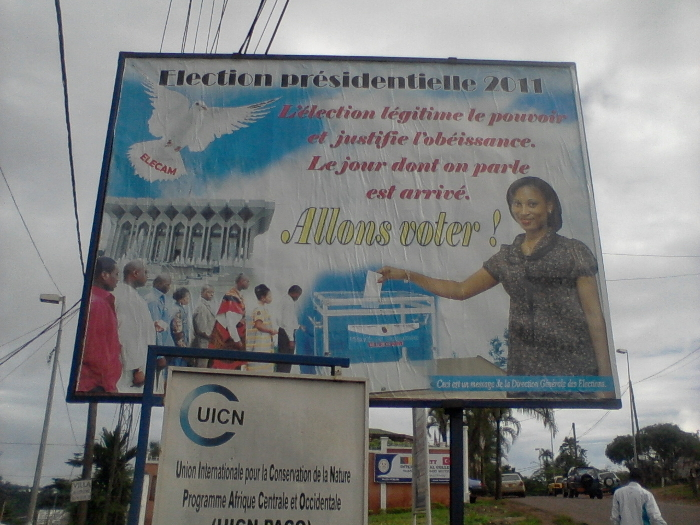
\includegraphics{img/Wahlen.jpg}
\caption{Ein Plakat der staatlichen Wahlkommission in Jaunde. Auffällig
ist hier die Feststellung, wonach Wahlen die Macht legitimieren und die
Notwendigkeit des Gehorsams (gegenüber den Herrschenden) rechtfertigen.
Bildquelle: Foto des Autors.}
\end{figure}

Kaum besser steht es um die gesellschaftliche Anerkennung der
bibliothekarischen Berufe. In vielen Schulen, aber nicht nur dort, wird
mancher leistungsschwache Mitarbeiter \enquote{zur Erholung} in die
Bibliothek versetzt. Generell genügen die Gehälter der Mitarbeiter
oftmals nicht, um sich und der Familie ein bescheidenes Leben zu
sichern. Die Folgen davon sind häufige Abwesenheiten zwecks Nebenerwerb
bzw. wegen mangelnder Motivation. Hat man zudem das \enquote{Glück} als
Beamter angestellt zu werden, braucht es in der Regel zwei bis drei
Jahre, bis das erste Gehalt ausgezahlt wird. Einen Teil dieser
unfreiwilligen Wartezeit verbringt der Bittsteller dann nicht an seinem
Arbeitsplatz, sondern in der Hauptstadt mit dem Putzen unzähliger
Türklinken in diversen Ministerien. Über dieses Problem berichten nicht
nur Bibliotheksmitarbeiter, sondern auch andere angehende Beamte, wie
zum Beispiel Lehrer.

Auch bei der bibliothekarischen Ausbildung werden Unterschiede zur
\enquote{Norm} sichtbar. Die Studiengänge einiger Einrichtungen sind
unter anderem durch fehlenden Praxisbezug sowie veraltete Lerninhalte
gekennzeichnet. Zum Beispiel lernten angehende Dokumentare und
Bibliothekare noch 2013 in der staatlichen Ausbildungsstätte ESSTIC,
dass es in Deutschland zwei Nationalbibliotheken gibt, eine davon in der
DDR (!). Des Weiteren endete ein Kurs zum Thema \enquote{Multimedia in
der Bibliothek} mit der Erwähnung der Video-Disc als neueste Entwicklung
auf diesem Gebiet.\footnote{Die beiden hier genannten Beispiele
  entstammen den Vorlesungsskripten einer Kollegin, die seit 2013 einen
  berufsbegleitenden Fernstudiengang zur Erlangung einer \emph{Licence
  Professionnelle} an der ESSTIC (École Supérieure des Sciences et
  Techniques de l'Information et de La Communication) absolviert. Sie
  stellen sicherlich Extremfälle dar, deuten aber grundsätzlich auf
  veraltete Lehrinhalte hin.} In der Tat sind die Vorlesungen mancher
Dozenten kaum mehr als die Zusammenstellung ihrer eigenen, während der
Studienzeit angefertigten Mitschriften.

Was Projekte im Bibliotheksbereich betrifft, so gibt es hier kaum
Unterschiede zu anderen gesellschaftlichen Bereichen im Land.
Protokollarische Details und die Dicke von zugestanden Geldumschlägen
erscheinen im Alltag wichtiger als das eigentliche Projektziel.
Angesichts der gesellschaftlichen Bedeutung von Essenseinladungen
verwundert es auch nicht, dass die Qualität und Quantität der kostenlos
angebotenen Speisen und Getränke mitunter über den Erfolg oder
Misserfolg einer organisierten Weiterbildungsveranstaltung entscheidet.

Die Ergebnisse solcher Projekte und Workshops lassen sich dann
gegebenenfalls an der Größe der entstandenen Ruinen messen. So gibt es
zum Beispiel in Marua eine aus einem internationalen Projekt heraus
entstandene öffentliche Bibliothek zu bewundern, die irgendwann vor
Jahren schlichtweg von Mitarbeitern und Besuchern verlassen wurde. Seit
diesem Tag warten Bücher, Regale, Stühle und Tische darauf, unter einer
dicken Staubschicht begraben zu werden, um dann womöglich irgendwann in
der Zukunft Gegenstand einer archäologischen Ausgrabung zu werden.
Wohlgemerkt, es handelt sich um die zentrale Öffentliche Bibliothek für
Marua und die Region Extrême-Nord, immerhin ein Gebiet mit über drei
Millionen Einwohnern!\footnote{Institut National de la Statistique du
  Cameroun: \emph{La Population du Cameroun en 2010}. o.J.
  \url{http://statistics.cameroon.org/news.php?id=18} (besucht am
  25.10.2014).} Marua ist dabei leider kein Einzelfall. Die Tageszeitung
\enquote{Mutations} berichtete in ihrer Ausgabe vom 14. Oktober 2014
darüber, dass es in Bertua, immerhin Hauptort der flächenmäßig größten
Region Est, derzeit keine einzige Bibliothek gäbe. Der Autor der
\enquote{Mutations} bezieht sich hierbei im Wesentlichen auf die dort
ebenfalls geschlossene Öffentliche Bibliothek. Über die Existenz einiger
kleinerer Bibliotheken scheint er hingegen nicht informiert zu sein.

\begin{figure}[htbp]
\centering
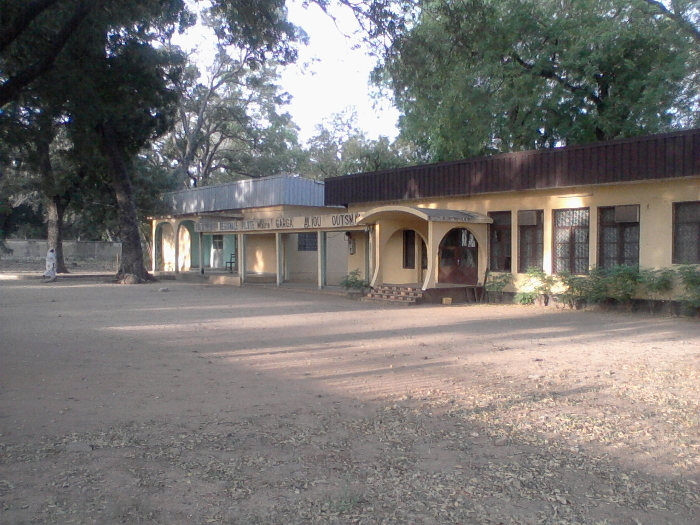
\includegraphics{img/Maroua2.jpg}
\caption{Die Garga-Aliou-Outsman-Bibliothek in Maroua. Die zentrale
Öffentliche Bibliothek für die Stadt Marua und die Region Extrême-Nord
ist seit mehreren Jahren geschlossen. Bildquelle: Foto des Autors.}
\end{figure}

\begin{figure}[htbp]
\centering
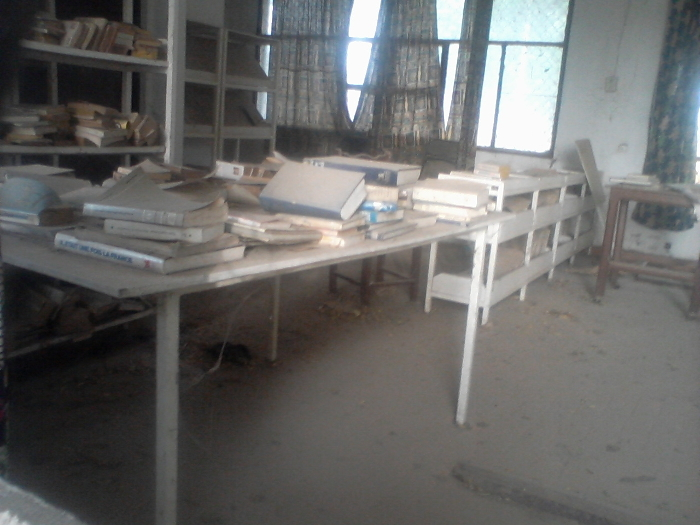
\includegraphics{img/Maroua1.jpg}
\caption{Die Garga-Aliou-Outsman-Bibliothek in Maroua. Ein Blick durchs
Fenster. Bildquelle: Foto des Autors.}
\end{figure}

\begin{figure}[htbp]
\centering
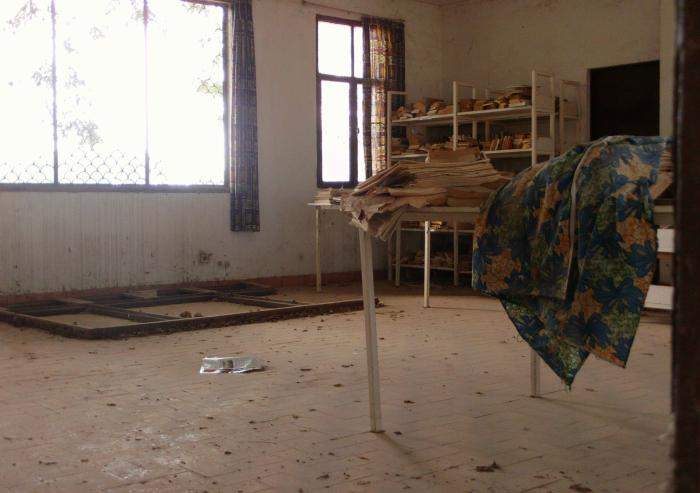
\includegraphics{img/Maroua3.jpg}
\caption{Die Garga-Aliou-Outsman-Bibliothek in Marua. Noch ein Blick
durchs Fenster. Bildquelle: Foto des Autors.}
\end{figure}

Angesichts dieser bisher beschriebenen Umstände mag es wenig verwundern,
dass die Nationalbibliothek des Landes seit fast 10 Jahren für die
Öffentlichkeit geschlossen ist und der seit 1973 Jahren existierende
nationale Bibliotheksverband ABADCAM (Cameroon Association of
Librarians, Archivists, Documentalists and Museographers) erst 2010 im
Rahmen des IFLA-BSLA-Programms\footnote{IFLA: \emph{BSLA Country
  Project: Cameroon}
  \url{http://www.ifla.org/bsla/country-reports/cameroon} (besucht am
  11.10.2014).} reanimiert wurde.

\section*{Ein Erklärungsversuch}\label{ein-erkluxe4rungsversuch}

Es wäre langweilig und wenig nutzbringend, sich weiter bei der
Aufzählung von Problemen aufzuhalten, die --- jedes für sich allein
genommen --- sicherlich auch in anderen Ländern festgestellt werden
können.\footnote{So hat zum Beispiel der Autor im August 2013 die
  Webauftritte der Nationalbibliotheken von 50 afrikanischen Ländern
  untersucht. Von diesen hatten 22 Länder eine Nationalbibliothek mit
  Webpräsenz. 16 dieser Webpräsenzen wurden seit 2010 mindestens einmal
  inhaltlich aktualisiert. Auf sechs Webpräsenzen bestand die
  Möglichkeit einer OPAC-Recherche. Dabei handelte es sich mit Kenia,
  Malawi, Mauritius, Namibia, Rwanda und Südafrika jeweils um Länder, in
  denen Englisch Amtssprache ist.} Generell ersichtlich wird allerdings
ein systematisches Abweichen vom Normalen, wobei die nicht erfüllten
Normen außerhalb des Landes definiert werden. Betrachtet man folglich
das Bibliothekswesen in Kamerun unter dem Gesichtspunkt, wie \enquote{es
eigentlich sein müsste}, bleiben Enttäuschungen nicht aus. Von den
beteiligten Akteuren vor Ort hört man jedoch in Bezug auf diesen oder
jenen Umstand immer wieder die Aussage: \enquote{C'est normal
!}\footnote{\enquote{Das ist normal!}} Allein diese ständig
wiederkehrende Floskel deutet bereits darauf hin, dass die extern
aufgestellten Normen mit denjenigen Normen, wie sie im Land selbst
definiert und von den beteiligten Akteuren wahrgenommen werden, nicht
übereinstimmen. Ganz offensichtlich befolgen viele Akteure im
kamerunischen Bibliothekswesen gänzlich andere Normen, wobei sie daran
durch ihre jeweils Aufsicht führenden Einrichtungen kaum behindert
werden.

Konkret führt dies zu der These, wonach das aus Europa bzw. Nordamerika
eingeführte Konzept der Bibliothek in Kamerun vielerorts abgeändert und
den Bedürfnissen von einigen der beteiligten Stakeholder angepasst
wurde. Diese Umwandlung erfolgte an einigen Orten so erfolgreich, dass
die ursprüngliche Funktionalität der \enquote{Bibliothek} nahezu
komplett dahinter verschwand. Im Extremfall berechtigt das Vorhandensein
eines angestaubten Regals mit einigen unattraktiven -- und daher noch
nicht gestohlenen -- Büchern zum Bezug eines regelmäßigen
Beamteneinkommens nebst der Aussicht auf Dienstreisezulagen und ab und
an anfallenden Projektgeldern. Im Normalfall ist der Extremfall ein
erstrebenswertes Ziel, wobei es dann auch gerne noch ein paar Regale
mehr sein dürfen.

In diesem Sinne stellt diese Art von Organisation eine Alternative zum
importierten und scheinbar universell geltenden Bibliothekskonzept dar,
freilich ohne dass die in Europa und Nordamerika definierten klassischen
Funktionen einer Bibliothek darin noch irgendwie ernsthafte Beachtung
fänden.

\begin{figure}[htbp]
\centering
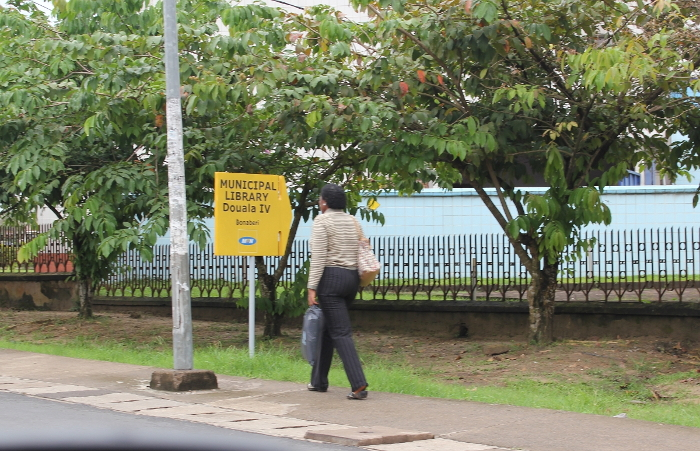
\includegraphics{img/LibDuala.jpg}
\caption{Ein Hinweisschild in Duala. Die Perspektive wollte es so, dass
dieses Schild in Richtung eines scheinbar unüberwindlichen Zaunes zeigt.
Als der Autor knapp ein Jahr später wieder vorbeikam, war vom Schild
nichts mehr zu sehen. Der Ort liegt in unmittelbarer Nähe zur
Wuri-Brücke in Duala, welche laut nicht näher belegbaren Angaben täglich
von über 1 Million Personen benutzt werden soll. Bildquelle: Foto des
Autors.}
\end{figure}

An dieser Stelle sei vor Missverständnissen gewarnt. Die hier
beschriebenen Fälle mögen vielleicht für die Mehrzahl der mit dem
Begriff \enquote{Bibliothek} umschriebenen Einrichtungen in Kamerun
zutreffen, für die Gesamtheit stimmt dies nicht. Es gibt sehr wohl
ernsthafte Bibliotheksprojekte mit engagierten Kolleginnen und Kollegen,
die dort ihre Angebote den Nutzern zukommen lassen. Es würde sich sicher
lohnen, die möglicherweise gemeinsamen Voraussetzungen für diese, von
außen betrachtet, wünschenswerte Praxis mit wissenschaftlichen Methoden
näher zu untersuchen. Als eine erste Hypothese bietet sich eine
angenommene Korrelation zwischen \enquote{erfolgreichen} Bibliotheken
und einer gewissen finanziellen Unabhängigkeit der jeweiligen
Verantwortlichen an.

Und auch ein weiteres Missverständnis muss hier geklärt werden. Das
eventuell anzuprangernde Verhalten der Mehrzahl der Kollegen und
Kolleginnen ist nicht etwa persönliche Unfähigkeit oder -- noch
schlimmer -- einer gruppenspezifischen Unfähigkeit als
\enquote{Afrikaner} geschuldet. Vielmehr handeln die jeweiligen Kollegen
streng rational, nämlich auf den Vorteil für sich selbst und für
Mitglieder ihrer Netzwerke ausgerichtet. Besagte Netzwerke können sich
ethnisch, religiös oder aber zum Beispiel auf der Basis von
Altersklassen konstituieren. Die Integration in diese Netzwerke
entscheidet in den Augen der Beteiligten weit stärker über deren
persönlichen Zukunftsperspektive, als dies ein abstrakt vermittelter
gesamtgesellschaftlicher Nutzen von Bibliotheken vermag.

\begin{figure}[htbp]
\centering
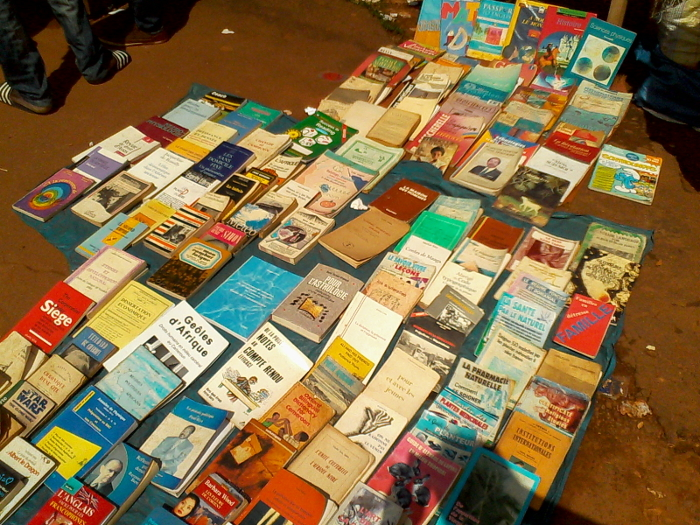
\includegraphics{img/LibrairiePoteau1.jpg}
\caption{Eine Straßenbibliothek in Jaunde. Die sogenannten
\enquote{Librairies de Poteau} sind am ehesten noch mit Leihbibliotheken
vergleichbar. Leser treten hier sowohl als Käufer als auch Verkäufer
auf. Von der Differenz lebt der Händler. Bildquelle: Foto des Autors.}
\end{figure}

\begin{figure}[htbp]
\centering
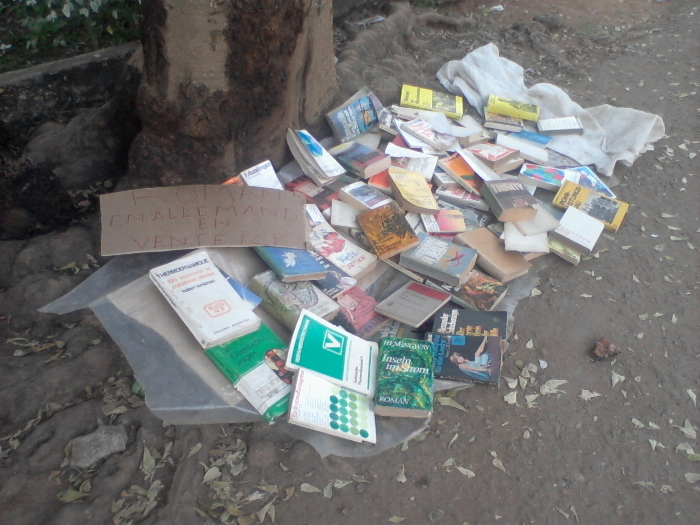
\includegraphics{img/LibrairiePoteau2.jpg}
\caption{Bildunterschrift: Eine weitere Straßenbibliothek in Jaunde. In
diesem Fall sollte eine private Sammlung deutscher Titel auf der dem
Goethe-Institut gegenüber liegenden Straßenseite zum Verkauf gebracht
werden. Bildquelle: Foto des Autors.}
\end{figure}

\begin{figure}[htbp]
\centering
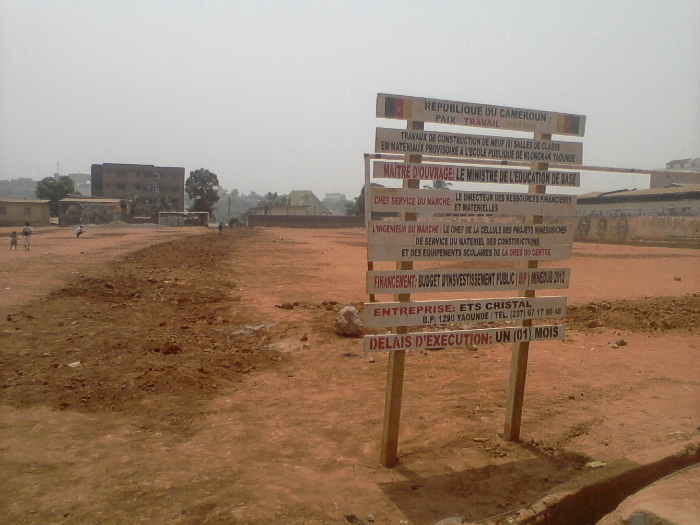
\includegraphics{img/bundesliga.jpg}
\caption{Eine verhinderte Baustelle. Im sogenannten Bundesliga-Stadium,
einem der besseren Bolzplätze in Jaunde, sollte Anfang 2013 die
Erweiterung einer benachbarten staatlichen Grundschule gebaut werden.
Die Anwohner wehrten sich, indem sie die tagsüber angelegten Gräben
nachts wieder zuschütteten. Die Auseinandersetzung entbehrt nicht einer
gewissen Symbolik. Bildquelle: Foto des Autors.}
\end{figure}

Um es noch einmal klar zum Ausdruck zu bringen: Die meisten Bibliotheken
in Kamerun basieren auf der Übernahme eines scheinbar universellen -- in
Wirklichkeit jedoch hauptsächlich im neuzeitlichen Europa bzw.
Nordamerika generierten -- Konzepts von Bibliothek. Dieses Konzept wurde
und wird von einzelnen Stakeholdern aktiv und kreativ den eigenen
Bedürfnissen angepasst und zwar so, dass zentrale Funktionen des
ursprünglichen Konzepts an Bedeutung verlieren bzw. ganz aufgegeben
werden.

Radikal betrachtet unterscheidet sich dieses Verhalten nur wenig vom
deutschen Kleingartenbesitzer, der sich eine Buddhafigur zwischen die
Beete stellt. Hier wie dort, wird aktiv importiert, das heißt es werden
nur diejenigen Teile eines Konzepts übernommen, die für den
\enquote{Importeur} nützlich und sinnvoll erscheinen.\footnote{Wir gehen
  dabei davon aus, dass sich der durchschnittliche deutsche
  Buddhafigurenbesitzer nicht umfassend mit den religiösen Grundsätzen
  des Buddhismus identifiziert.} Es wäre vermessen und im Grunde
genommen Ausdruck einer kolonialen Denkweise, würde der
\enquote{Exporteur} auf die detailgetreue Übernahme seines Konzepts
beharren. Genau das ist jedoch leider in der Praxis noch viel zu häufig
der Fall.

In der Postkolonialismus-Debatte werden die hier beschriebenen Phänomene
dem Konzept der Hybridisierung zugeordnet. Homi K. Bhabha, auf den
dieses Konzept zurückgeht, sieht im Grenzbereich zwischen zwei Kulturen
Gestaltungsmöglichkeiten und Freiräume für Gruppen und Individuen im
Rahmen eines sogenannten \emph{Third Space.} Es handelt sich um einen
neu entstehenden Raum zwischen dem ersten Raum des globalen Nordens und
dem zweiten Raum des globalen Südens.\footnote{Bhabha, Homi K.:
  \emph{The Location of Culture}. 1994. London: Routledge.} Bhabha,
dessen biographischer Hintergrund ihn teilweise selbst zum Bewohner
dieses dritten Raumes macht, kann diesem überwiegend positive
Eigenschaften abgewinnen. Und zweifellos entwickeln die aufgeführten
Akteure in den kamerunischen Bibliotheken ihre Strategien und Freiräume
auf der Basis ihres Spiels zwischen den Kulturen. Ob sie jedoch zugleich
als Vermittler zwischen diesen Kulturen auftreten können und wollen
erscheint hingegen fraglich.

\section*{Vorschläge für die
Praxis}\label{vorschluxe4ge-fuxfcr-die-praxis}

Was bedeutet nun die hier aufgestellte These für die Praxis, genau
genommen für die aus der Perspektive des Außenstehenden erlebte Praxis?
Es wird hier schnell deutlich, dass die festgestellten Widersprüche in
der Strategie und dem Verhalten des \enquote{Exporteurs}
Berücksichtigung finden müssen. Es wird aber auch deutlich, dass diese
Widersprüche unter den jetzigen Bedingungen kaum aufgelöst werden
können. Die Beziehungen des ersten Raumes zum dritten Raum, zwischen
\enquote{Exporteur} und \enquote{Importeur}, sind in vielen Fällen zu
asymmetrisch, als dass sich dadurch viel Neues zu beiderseitigem Vorteil
entwickeln könnte. Trotzdem soll hier eine Sammlung von Prämissen und
Handlungsmaximen zur Diskussion gestellt werden:

\begin{enumerate}
\def\labelenumi{\arabic{enumi}.}
\item
  Das zur Diskussion stehende Konzept einer Bibliothek als Ort des
  Sammelns, Bewahrens, Zugänglichmachens und Vermittelns von Information
  mag nach der im globalen Norden vorherrschenden Theorie universell
  gültig erscheinen. Es entspringt jedoch einer spezifischen
  kulturhistorischen Entwicklung und ist deshalb in der Praxis nicht
  ohne weiteres auf andere Kulturen übertragbar. Erst recht nicht dort,
  wo die kollektive Erinnerung an einem oftmals gewaltsamen,
  asymmetrischen Kulturaustausch, wie es dem kolonialen System zu eigen
  ist, noch lebendig ist.
\item
  Die zweifellos existierenden praktischen Vorteile des westlichen
  Konzepts von Bibliothek können und sollen beworben werden. Ein
  bedingungsloses Beharren auf deren notwendige praktische Umsetzung ist
  jedoch fehl am Platze. Als solche Vorteile seien hier unter anderem
  genannt: die Speicherung von Informationen unabhängig von menschlichen
  Übermittlern, der verbesserte und möglichst frei gestaltete Zugang zu
  diesen Informationen sowie das Auftreten von Bibliotheken als Orte des
  informellen Lernens.
\item
  Die Entwicklung eines lokal angepassten Konzepts mit unbedingter und
  maßgeblicher Beteiligung der betroffenen Akteure sollte aufmerksam
  beobachtet und gegebenenfalls auch gefördert bzw. unterstützt werden.
  Dabei kommt der Förderung des fachlichen Dialogs auf nationaler und
  internationaler Ebene eine besondere Bedeutung zu. Der Dialog bietet
  gute Voraussetzungen für gangbare Lösungen unter rechtzeitigem
  Ausschluss von Fehlentwicklungen. Es ist jedoch klar, dass die im
  Dialog ausgehandelten Verfahren irgendwann auch in die Praxis
  umgesetzt werden sollten.
\item
  Die beteiligten Kollegen und Kolleginnen vor Ort müssen als
  selbstständig und rational handelnde Akteure in ihrem jeweiligen
  Kontext wahrgenommen werden. Obwohl es eigentlich eine
  Selbstverständlichkeit ist, verdient es dieser letzte Satz, besonders
  betont zu werden.
\item
  Einmischung von außen im Sinne von bewussten oder unbewussten Vorgaben
  sollte vermieden werden. Dabei werden häufig gerade die Auswirkungen
  von unbewussten Vorgaben unterschätzt. So führt zum Beispiel die an
  die Bibliotheksmitarbeiter signalisierte Erwartungshaltung, was als
  gute Bibliotheksarbeit gilt und was nicht, nicht selten zu
  vorauseilendem Gehorsam beim Partner. Das Ergebnis dessen ist, dass
  der eigentliche Kern des Problems in der Diskussion nicht angesprochen
  wird. In diesem Sinne wäre das Wagen von mehr Abstand ein denkbarer
  Weg zur Entwicklung von selbstständigen und tragfähigen lokal
  entwickelten Konzepten. \emph{Abstand} bedeutet in diesem Sinne zum
  einen den freiwilligen Verzicht auf latente bzw. manifeste Einmischung
  der stärkeren Seite in Bezug auf die sich anbietenden
  Problemlösungsoptionen. \emph{Abstand} bedeutet aber auch, dass die
  scheinbar schwächere Seite sich die Möglichkeit offen hält, eigene
  Problemlösungsstrategien zu entwickeln. Es ist jedoch fraglich, ob
  diese beiden hier angesprochenen Aspekte von \emph{Abstand} angesichts
  der materiellen und damit machtpolitischen Ungleichgewichte überhaupt
  in der Praxis umgesetzt werden können.
\end{enumerate}

Probleme bei der Sammlung, Aufbewahrung, Zugänglichmachung und
Vermittlung von Informationen sind auch in der kamerunischen
Gesellschaft zweifellos vorhanden. Ein Rückgriff auf vorkoloniale Formen
des Informationsmanagements scheint nicht möglich. Die hundertprozentige
Übernahme westlicher Konzepte erweist sich hingegen als eine Illusion.
Die Lösung dürfte in der Entwicklung angepasster Konzepte mit Blick auf
den gesamtgesellschaftlichen Nutzen sowie in der Unterstützung durch
Staaten entwickelter Bibliothekssysteme liegen. Die Initiative hierzu
muss aus dem Inneren der kamerunischen Gesellschaft heraus erfolgen.
Dazu wiederum muss den Akteuren mehr intellektuelle Eigenständigkeit
zugebilligt werden. Folglich muss die Ausbildung gemäß der aktuellen
Praxis und des wissenschaftlichen Diskurses angepasst werden.

Es ist interessant zu sehen, wie in den letzten Jahren Forderungen nach
mehr intellektueller Eigenständigkeit (oder besser Unabhängigkeit)
massiv in die gesellschaftlichen Diskussionen Einzug gehalten haben.
Hauptsächlich spielen diese Forderungen im Rahmen der eingangs erwähnten
kommenden politischen Auseinandersetzungen eine Rolle. Es ist jedoch
noch nicht abzusehen, inwiefern sie die reale gesellschaftliche
Entwicklung beeinflussen und ob sie auch das Bibliothekswesen erreichen
werden. Unter der Voraussetzung, dass es dabei friedlich zugeht, wäre
dies zu wünschen.

%autor
\begin{center}\rule{0.5\linewidth}{\linethickness}\end{center}

\textbf{Uwe Jung}
(\href{mailto:jung.uwe@gmail.com}{\nolinkurl{jung.uwe@gmail.com}})
arbeitet seit 2005 am Goethe-Institut Kamerun als Leiter des Bereichs
Information und Bibliothek. Er kann auf ein abgeschlossenes
Magister-Studium der Afrikawissenschaften sowie einen erfolgreich
absolvierten berufsbegleitenden Master-Studiengang BIW, beide an der
Humboldt-Universität zu Berlin, verweisen.

\end{document}
